\documentclass[a4paper]{article}
\usepackage[T1]{fontenc}
\usepackage[utf8]{inputenc}
\usepackage[italian]{babel}
\usepackage{enumitem}
\usepackage{graphicx}
\usepackage{makecell}
\graphicspath{{./images/}}
\usepackage{tabularx}
%\usepackage{geometry} 
    %\geometry{a4paper,top=3cm,bottom=3cm,left=3.5cm,right=3.5cm,% heightrounded,bindingoffset=5mm}
    
    \begin{document}
    
    \author{Manuel Trivilino, Davide Salaorni, Luca Terracciano}
    
    \title{\Large Data4Help\\
    \Large RASD Requirements Analysis and Specification Document
    }
    
    \maketitle
    \newpage
    
    \tableofcontents
    \newpage
    
    \section{Introduction}
    
    \subsection{Purpose}
    
    \subsection{Scope}
    
    \paragraph{Description of the given problem}
    
    \paragraph{}
    TrackMe is a company that develops software-based services for third parties and for consumers. The main service is called Data4Help.
     Data4Help is a service that allows third parties to monitor the location and the health status of individual, it handles a policy of permissions for each user and collects individual’s data from their personal devices.
    The service supports the registration of individuals who, by registering, agree that TrackMe acquires their data. After registration, these third parties can request:
    
    \begin{itemize}
        \item Access to the data of some specific individuals (we can assume, for instance, that they know an 
        individual by his/her social security number or fiscal code in Italy). In this case, TrackMe passes 
        the request to the specific individuals who can accept or refuse it.
        
        \item Access to anonymized data of groups of individuals (for instance, all those living in a certain 
        geographical area, all those of a specific age range, etc.). These requests are handled directly 
        by TrackMe that approves them if it is able to properly anonymize the requested data. For 
        instance, if the third party is asking for data about 10-year-old children living in a certain street 
        in Milano and the number of these children is two, then the third party could be able to derive 
        their identity simply having people monitoring the residents of the street between 8.00 and 
        9.00 when kids go to school. Then, to avoid this risk and the possibility of a misuse of data,
        TrackMe will not accept the request. For simplicity, we assume that TrackMe will accept any 
        request for which the number of individuals whose data satisfy the request is higher than 
        1000.
    
    \end{itemize}
    
    \paragraph{}
    As soon as a request for data is approved, TrackMe makes the previously saved data available to the 
    third party. Also, it allows the third party to subscribe to new data and to receive them as soon as 
    they are produced.
    TrackMe develops itself two third-party services: AutomatedSOS and Track4Run.
    
    \paragraph{Goals}
    
    \begin{enumerate}[label*={G.\arabic*}]
        
        %Data4Help
        
        \item Allow users' registration.
        \begin{enumerate}[label*=.\arabic*]
            \item Registration can be done as individual user.
            \item Registration can be done as third party.
        \end{enumerate}
        
        \item Third parties can request for anonymized data.
    
        \item Third parties can subscribe to the service in order to periodically receive new data.
            
        \item Third parties can receive for a individual user's data.
        
        %AutomatedSOS
        \item Users' health status is continuously checked in AutomatedSOS and in case of it overcomes a certain threshold values an ambulance is called within 5 seconds.
        
        %Track4Run
        \item Users can organize a run.
        \item Users can enroll to a run.
        \item Users can be spectators of a run seeing the partecipants' position on a map.
        
    \end{enumerate}
    
    \subsection{Definitions, Acronyms, Abbreviation}
    
    
    \subsection{Revision History}
    
    \subsection{Reference Documents}
    
    \subsection{Document Structure}
    
    \section{Overall Description}
    
    \subsection{Product Perspective}
    
    \begin{figure}[h!]
        \centering
        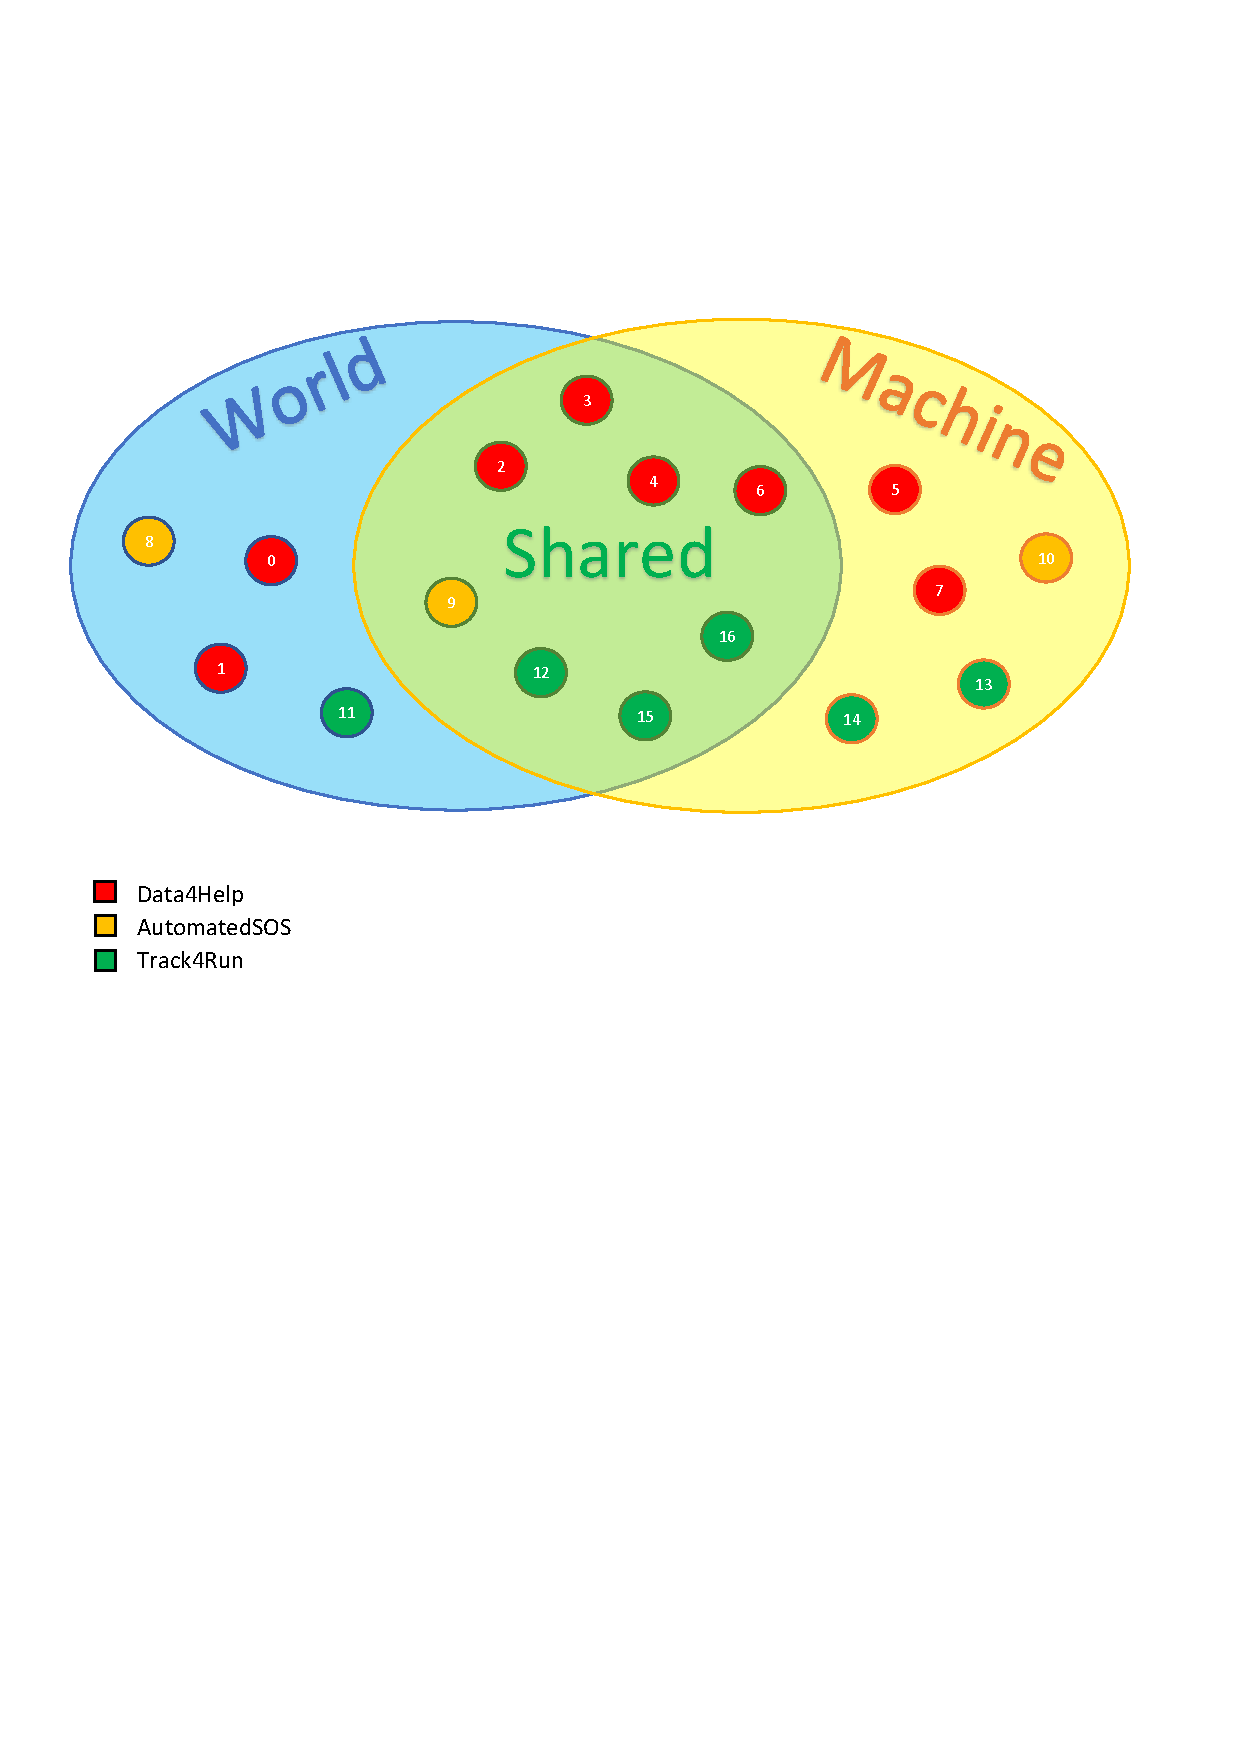
\includegraphics[width=\linewidth]{worldMachineShared-small}
        \caption{World, machine and shared phenomena.}
        \label{fig:my_label}
    \end{figure}
    
    
    \subsection{Product Functions}
    
    \subsection{User Characteristics}
    
    \paragraph{}The following actors are the users of the services offered by TrackMe. 
    
    
    \begin{itemize}
        \item User:  a person that is successfully registered to TrackMe as consumer and allow to acquire anonymous data, eventually a client of third party services (i.e. AutomatedSOS, Track4Run) that allows even personal data.
        
        \item Third Parties:  a company or a person who is registred to TrackMe as "Third party" that access to anonymous and can require to access to individual data.
        
    \end{itemize}
    
    \subsection{Assumption, Dependencies and Constraints}
    
    \subsubsection{Domain Assumptions}
    
    
    \begin{enumerate}[label={[D.\arabic*]}]
        
        \item The data collected from the devices (position and health status) are reliable, accurate and in real time.
        \item The personal information given by the user (age, address, gender...) are correct and the account is not used by other people. 
        \item Ambulance call and information about patients' status and position are correctly dispatched to the ambulance contact center.
        \item Information and data (places, maps, paths, etc.) received from external services are correct are reliable.
        
    \end{enumerate}
    
    
    \section{Specific Requirements}
    
    \subsection{External Interface Requirements}
    
    \subsubsection{User Interfaces}
    
    %MOCKUP
    
    
    \subsubsection{Hardware Interfaces}
    
    \paragraph{Data4Help:} is the main service offered by TrackMe. It is a software based service and its function is to collect data from the users, make them available to third parties who require for it and handle the permissions between users and third parties. The service can be accessible from a web browser or from the smartphone app.
    
    \paragraph{AutomatedSOS:} to guarantee its non-intrusive SOS services it needs to collect personal information from a mobile device (smartphone, smartwatche, smart bands linked to the smartphone etc.) with GPS and a cardiac pulse sensor or other sensors that let to monitor the user's health status.
    
    \paragraph{Track4Run} requires a mobile devices (smartphone, smartwatch, smart band linked to the smartphone) with GPS to keep track of the runners' position.
    
    \subsubsection{Software Interfaces}
    
    \paragraph{Data4Help:} the system needs to transfer data with users and thirds parties and keep track of the permissions the interfaces needed are:
    \begin{itemize}
        \item REST API to communicate and transfer data on the web.
        \item mySQL DBMS to manage the database.
    \end{itemize}
    
    \paragraph{AutomatedSOS:} the system needs to manage the communication between the users and Data4Help, to analyze the data and to communicate with the ambulance dispatscher. The interfaces needed are:
    
    \begin{itemize}
        \item REST API to communicate and transfer data on the web.
        \item Interface with Push service to a safe connection to send reliable messages to require health care to the ambulance dispatcher.
    \end{itemize}
    
    \paragraph{Track4Run:} the system needs to manage the run events with the respective runners and spectators and let the spectators watch the run events on the map. The interfaces needed are:
    
    \begin{itemize}
        \item REST API to communicate and transfer data on the web.
        \item interface with the Google Maps API to manage the map for the runs.
    \end{itemize}
    
    
    \subsubsection{Communication Interfaces}
    
    The system is based on the Client-Server architecture, in particular the communication between the different actors and elements of the system (Users-Data4Help, Third Parties-Data4Help, Users-AutomatedSOS, Users-Track4Run) is based on: the REST API to make requests, the AJAX API to transfer data.
    This is a possible coniguration of the system:
    
    \subsection{Functional Requirements}
    
    \begin{enumerate}[label*=\bf{G.\arabic*}]
        
        %Data4Help
        \item \textbf{Allow users’ registration.}
        \begin{enumerate}
            \item [D.2] The personal information given by the user (age, address, gender...) and the third parties are correct and the account is not used by other people. 
        \end{enumerate}
        
        \begin{enumerate}[label*=\bf{.\arabic*}]
            \item \textbf{Registration can be done as individual user.}
            \begin{enumerate}
                \item [R.1] People can create a user account selecting username, password, giving personal informations (age, address,gender) and allow to share their anonymized data.
                
            \end{enumerate}
            
            \item \textbf{Registration can be done as third party.}
            \begin{enumerate}
                \item [R.2] It is possible to create a third party account selecting username and password and giving the company main information.
            \end{enumerate}
        \end{enumerate}
        
        \item \textbf{Third parties can receive anonymized data.}
                
        \begin{enumerate}
            \item [R.3] Data4Help allows third parties to request anonymized data acquired from a filtered group of users (by age, gender, address, etc.).
            \item [R.4] Data4Help collects data from registered users and gives access to third parties only if the number of individuals whose data satisfy the request is higher than 1000.
            \item [D.2] The personal informations given by the user (age, address, gender...) and the third parties are correct and the account is not used by other people.
        \end{enumerate}
            
            
        \item \textbf{Third parties can subscribe to the service in order to periodically receive new data.}
        
        \begin{enumerate}
            \item [R.5] Data4Help allows third parties to join the subscription service for an indeterminate period and then, in case, unsubscribe from that.
            \item [R.6] Data4Help provides new data, checking each time if groups data satisfy the given constraint (number of individuals not lower than a thousand).
            \item [R.7] Data4Help keeps track of the associations between third parties subscriptions and the required group data.
        \end{enumerate}
        
        
        \item \textbf{Third parties can receive specific person's data.}
                
        \begin{enumerate}
            \item[R.8] Data4Help allows third parties to require specific person's data. 
            \item [R.9] Data4Help forwards requests from third parties to the demanded users which can accept or refuse to share their own personal data.
            \item [R.10] Data4Help keeps track of the connections between a specific user and the third parties which can access to his/her data.
            \item [R.11] Data4Help allows third parties to have access to demanded users' data each time they need them.
        \end{enumerate}
                
            
        %AutomatedSOS
        \item \textbf{Users' health status is continuously checked in AutomatedSOS and if it is below a certain threshold values an ambulance is called within 5 seconds and sent to the user's position.}
    
        \begin{enumerate}
            \item [D.1] The data collected from the devices (position and health status) are reliable, accurate and in real time.
            \item [R.12] Users' health and position information received by Data4Help are analyzed and compared with the threshold values.
            \item [R.13] In case of emergency (the health status values overcome the threshold) a request for an ambulance is sent to the ambulance dispatcher in 5 seconds, containing the user's information.
            \item [D.3] Ambulance call and information about patients' status and position are correctly dispatched to the ambulance contact center.
        \end{enumerate}
        
        %Track4Run
        \item \textbf{Users can organize a run.}
        
        \begin{enumerate}
            \item [R.14] Users select the day, the hour at which the run begins, the starting point, the ending point and the path for the run.
            \item [R.15] The run event is stored in the system in order to be managed during its lifecycle.
            \item [D.4] Information and data (places, maps, paths, etc.) received from external services are correct and reliable.
        \end{enumerate}
        
        \item \textbf{Users can organize a run.}
        
        \begin{enumerate}
            \item [R.16] Users can browse among the available runs and see their information.
            \item [R.17] Users can choose a run and register to it as a runners.
  % NON-FUNCTIONAL         \item [R.12] Users can choose to see the available runs filtering them by city and/or date. 
            \item [R.18] The system saves the enrolled users as runners and keeps track of the association with the run event.
        \end{enumerate}
        
        \item \textbf{Users can be spectators of a run seeing the participants' position on a map.}
        
        \begin{enumerate}
            \item [R.14] The system keeps track of all the enrolled runners' position during the run.
            \item [R.15] Users who require to watch a run are saved as spectators to the run event.
            \item [R.16] Track4Run offers the possibility to see the run live through a map.
            \item [D.4] Information and data (places, maps, paths, etc.) received from external services are correct and reliable.
        \end{enumerate}
        
    \end{enumerate}
    
    
    \paragraph{Use cases}

\subsubsection{User's sign up}
\begin{center}
    \begin{tabular}{ l || p{8cm} ||}
        \bf{ACTORS} & User \\ 
        \hline
        \bf{ENTRY CONDITIONS} & No entry condition needed  \\ 
        \hline
        \bf{EVENTS FLOW} & \begin{itemize}[noitemsep, topsep=0cm, leftmargin=*] \vspace{-0.2cm}
            \item[1.] User opens Data4Help app and press “Sign Up” button.
            \item[2.] User inserts personal informations (name, address, age, gender, fiscal code).
            \item[3.] User selects email and password.
            \item[4.] User allows terms of conditions to share anonymized data with Data4Help.
            \item[5.] User completes the registration.
            \item[6.] The system saves the new account.
        \end{itemize}\\ 
        \hline
        \bf{EXIT CONDITIONS} & The user is successfully registered and his/her data can be collected by Data4Help, he/she is redirected to the user page\\ \hline
        \bf{EXCEPTIONS} & \begin{itemize}[noitemsep, topsep=0cm, leftmargin=*] \vspace{-0.2cm}
            \item[1.] The user doesn’t fill all the mandatory fields with valid data.
            \item[2.]The inserted email is already used by another user.
            \item[3.] The user doesn’t allow the term of condition and he/she can’t complete the registration.
        \end{itemize}
        \\ \hline \hline
    \end{tabular}
\end{center}

\vspace{1cm}

\subsubsection{One-time request for anonymous data set}
\begin{center}
    \begin{tabular}{l || p{8cm} ||}
        \bf{ACTORS} & Third Party \\ \hline
        \bf{ENTRY CONDITIONS} & This use case start when the third party is registered, successfully logged in to Data4Help and is connected to the web page.\\ \hline
        \bf{EVENTS FLOW} & \begin{itemize}[noitemsep, topsep=0cm, leftmargin=*] \vspace{-0.2cm}
            \item[1.] The Third Party click on "Data Request" button.
            \item[2.] The Third Party selects to require anonymous data with a one-time request.
            \item[3.] The Third Party selects the filter that must be applied to gather users.
            \item[4.] The system checks if the request can be accepted to guarantee the users' anonymity or not.
            \item[5.] Third party receives the confirmation to the request.
        \end{itemize}
        \\ \hline
        \bf{EXIT CONDITIONS} & The request is accepted and anonymized data are sent to the Third Party.\\ \hline
        \bf{EXCEPTIONS} & The number of users satisfying the filter is smaller than 1000, then the request is refused. 
        \\ \hline \hline
    \end{tabular}
\end{center}

\vspace{1cm}

\subsubsection{Subscription to anonymous data}
\begin{center}
    \begin{tabular}{l || p{8cm} ||}
        \bf{ACTORS} & Third Party \\ \hline
        \bf{ENTRY CONDITIONS} & This use case start when the third party is registered, successfully logged in to Data4Help and connected to the web page.\\ \hline
        \bf{EVENTS FLOW} & \begin{itemize}[noitemsep, topsep=0cm, leftmargin=*] \vspace{-0.2cm}
            \item[1.] The Third Party clicks on "Data Request" button.
            \item[2.] The Third Party selects to require anonymous data with a subscription request.
            \item[3.] The Third Party selects the filter that must be applied to gather users.
            \item[4.] The system checks if the request can be accepted to guarantee the users' anonymity or not.
            \item[5.] The Third Party receives the confirmation to the request.
            \item[6.] The Third Party is periodically notified with new anonymous data about the selected users' group. 
        \end{itemize}
        \\ \hline
        \bf{EXIT CONDITIONS} & The Third Party decides to unsubscribe from the service and stops to receives periodical updates.\\ \hline
        \bf{EXCEPTIONS} &\begin{itemize}[noitemsep, topsep=0cm, leftmargin=*] \vspace{-0.2cm}
            \item[1.] The number of users satisfying the filter is smaller than 1000, then the request is refused.
            \item[2.] During the service supply the number of users in the group decreases under 1000 entities, so the service is stopped.
        \end{itemize}
        \\ \hline \hline
    \end{tabular}
\end{center}


\vspace{1cm}

\subsubsection{Request for specific user's data}
\begin{center}
    \begin{tabular}{l || p{8cm} ||}
        \bf{ACTORS} & Third Party, User \\ \hline
        \bf{ENTRY CONDITIONS} & This use case start when the Third Party is registered, successfully logged in to Data4Help and connected to the web page.   \\ \hline
        \bf{EVENTS FLOW} & \begin{itemize}[noitemsep, topsep=0cm, leftmargin=*] \vspace{-0.2cm}
            \item[1.] The Third Party clicks on "Data Request" button.
            \item[2.] The Third Party selects the option " Require Individual Data".
            % Dubbio sul seguente punto
            \item[3.] The system sends a request to the users who want to use service offered by the Third Party.
            \item[4.] Once the user has allowed to acquire his/her personal data, a confirmation to the request is sent to the Third Party.
            % Dubbio se superfluo o meno
            \item[5.] The Third Party is redirected to the main page.
        \end{itemize}
        \\ \hline
        \bf{EXIT CONDITIONS} & The Third Party can require and access to user's personal data. \\ \hline
        \bf{EXCEPTIONS} & The user doesn't allow to share personal data and the system reject the request of the Third Party.
        \\ \hline \hline
    \end{tabular}
\end{center}

\vspace{1cm}

%AutomatedSOS
\subsubsection{Alert emergency status}
\begin{center}
    \begin{tabular}{l || p{8cm} ||}
        \bf{ACTORS} & User, Ambulance Contact Center \\ \hline
        \bf{ENTRY CONDITIONS} & This use case start when the user is registered and logged in to AutomatedSOS on his/her device, moreover has allowed the permission to share personal data with this third party. \\ \hline
        \bf{EVENTS FLOW} & \begin{itemize}[noitemsep, topsep=0cm, leftmargin=*] \vspace{-0.2cm}
            \item[1.] The system acquires the user's health data collected from his/her device.
            \item[2.] The system analyzes the data and notices that the health status is under the secure threshold.
            \item[3.] The system sends an ambulance request to the ambulance contact center within 5 seconds, reporting the user's health status and the position.
            \item[4.] The system send a warning to the user's device to notify that the health status is under the threshold and that an ambulance has been called to reach his/her position.
        \end{itemize}
        \\ \hline
        \bf{EXIT CONDITIONS} & The ambulance dispatcher sends a confirmation to the system that an ambulance has been sent to the user position. The system keep monitoring the user's health status.  \\ \hline
        \bf{EXCEPTIONS} & \begin{itemize}[noitemsep, topsep=0cm, leftmargin=*] \vspace{-0.2cm}
            \item[1.] The Ambulance contact center doesn't send any confirmation. The system sends again a request with the updated information until a confirmation is received or the health status comes back to safe values.
        \end{itemize}
        \\ \hline \hline
    \end{tabular}
\end{center}

\vspace{1cm}

%Track4Run
\subsubsection{Creation of a run event}
\begin{center}
    \begin{tabular}{l || p{8cm} ||}
        \bf{ACTORS} & User \\ \hline
        \bf{ENTRY CONDITIONS} & This use case start when the user is registered and logged in to Track4Run on his/her device, moreover has allowed the permission to share personal data with this third party.  \\ \hline
        \bf{EVENTS FLOW} & \begin{itemize}[noitemsep, topsep=0cm, leftmargin=*] \vspace{-0.2cm}
            \item[1.] The user select the "Create a run" button.
            \item[2.] The user choose the starting point, the ending point and the path on the map.
            \item[3.] The user selects the day and the starting time of the run event.
            \item[4.] The system confirms the run event creation to the user and saves it in the database.
        \end{itemize}
        \\ \hline
        \bf{EXIT CONDITIONS} & The run event is created and the track4Run users can enroll to the event.\\ \hline
        \bf{EXCEPTIONS} & \begin{itemize}[noitemsep, topsep=0cm, leftmargin=*] \vspace{-0.2cm}
            \item[1.] The selected path or the starting/ending point are unavailable for a run. The system let the user choose another one which is available.
        \end{itemize}
        \\ \hline \hline
    \end{tabular}
\end{center}

\vspace{1cm}

\subsubsection{Enrollment in a run}
\begin{center}
    \begin{tabular}{l || p{8cm} ||}
        \bf{ACTORS} & User \\ \hline
        \bf{ENTRY CONDITIONS} & This use case start when the user is registered and logged in to Track4Run on his/her device. Moreover has allowed the permission to share personal data with this third party and at least a run event has been already created. \\ \hline
        \bf{EVENTS FLOW} & \begin{itemize}[noitemsep, topsep=0cm, leftmargin=*] \vspace{-0.2cm}
            \item[1.] The user select the "Enroll to a run" button.
            \item[2.] The user selects the city that interests him/her.
            \item[3.] The system shows the list of available runs in the selected city.
            \item[4.] The user select the run event he /she wants to enroll.
            \item[5.] The system saves the user in the run event as a runner.
            \item[6.] The system notifies the user when the run is going to start.
        \end{itemize}
        \\ \hline
        \bf{EXIT CONDITIONS} & The user is correctly enrolled to the run event and can take part to it. \\ \hline
        \bf{EXCEPTIONS} & \begin{itemize}[noitemsep, topsep=0cm, leftmargin=*] \vspace{-0.2cm}
            \item[1.] The run event is already started. The user can't enroll the run, he/she is redirected to the run event's list.
        \end{itemize}
        \\ \hline \hline
    \end{tabular}
\end{center}

\vspace{1cm}

\subsubsection{Watch a run}
\begin{center}
    \begin{tabular}{l || p{8cm} ||}
        \bf{ACTORS} & User \\ \hline
        \bf{ENTRY CONDITIONS} & This use case start when the user is registered and logged in to Track4Run on his/her device,on the main page. Moreover has allowed the permission to share personal data with this third party and at least a run event has been already created. \\ \hline
        \bf{EVENTS FLOW} & \begin{itemize}[noitemsep, topsep=0cm, leftmargin=*] \vspace{-0.2cm}
            \item[1.] The user select the "View a run" button.
            \item[2.] The user selects the city that interests him/her. 
            \item[3.] The system shows the list of available runs in the selected city.
            \item[4.] The user select the run event he /she wants to watch.
            \item[5.] The system saves the user in the run event as a spectator.
        \end{itemize}
        \\ \hline
        \bf{EXIT CONDITIONS} & The user can watch on his/her device the map with the path and the runners positions updated in real time. \\ \hline
        \bf{EXCEPTIONS} & \begin{itemize}[noitemsep, topsep=0cm, leftmargin=*] \vspace{-0.2cm}
            \item[1.] 
        \end{itemize}
        \\ \hline \hline
    \end{tabular}
\end{center}
    
    \subsection{Performance Requirements}
    
    \paragraph{Data4Help} The system is designed to provide a large number of users and third parties moreover it is necessary to guarantee that the data is acquired, analyzed and made available to third parties in reasonable times. Especially individual data has to be provided to the third parties as soon they require them (periodically or even with real time updates).
    
    \paragraph{AutomatedSOS} This is a non-intrusive SOS service that needs to monitor the user health status in every moment. Once user's data are received from Data4Help the system must analyze the values and compare them with safe thresholds in a short time. If the values are under the fixed thresholds the system must warn the ambulance contact center in 5 seconds to send an ambulance to the user location.
    
    \paragraph{Track4Run} the system must be able to manage a large number of users enrolled in a single run event (the number of runners for a single run can be between less then 10 and almost 1000), a large number of run events for several cities and it must guarantee that the spectators can watch the runners' position on the map with a real time update.
    
    
    \subsection{Design Constraints}
    
    \subsubsection{Standards Compliance}
    
    Individual people to get access to Data4Help, AutomatedSOS and Track4Run services must sign in to Data4Help. By registering to Data4Help the user must allow the permissions to share anonymized data with Data4Help and third parties, unless he/she can't complete the registration.
    AutomatedSOS and Track4Run are third parties actors developed by TrackMe and, as such, they have to require to Data4Help the permission to receive individual data from the users.
    If an user wants to use AutomatedSOS and Track4Run services must accept the permissions to share individual data with them, unless their data can't be dispatched from Data4Help to the specific third partiy and the third party service can't be provided.
    
    \subsubsection{Hardware Limitations}
 \textbf{Data4Help} doesn't require specific hardware limitations for third parties. Users should use mobile devices with sensors useful for collecting data (GPS, cardiac pulse sensor, accelerometer, camera, light sensor) even if they are not strictly required. The only necessary requirement is that the device must have an internet connection (possibly fast):
    \begin{itemize}
        \item 3G/4G internet connection
    \end{itemize}
    
\noindent The hardware requirements for \textbf{AutomatedSOS} users' device, to collect the health information are:
    \begin{itemize}
        \item 3G/4G internet connection
        \item GPS
        \item Cardiac pulse sensor, other health sensors
    \end{itemize}
\noindent The hardware requirements for \textbf{Track4Run} users' devices are:
    \begin{itemize}
        \item 3G/4G internet connection
        \item GPS
        \item Device that supports Google maps API
    \end{itemize}
    
    \subsubsection{Any other Constraint}
    
    
    %Design constraints end
    
    \subsection{Software System Attributes}
    
    \subsubsection{Reliability}
    
    \subsubsection{Availability}
    
    \subsubsection{Security}
    
    \subsubsection{Maintainability}
    
    \subsubsection{Portability}
    
    \section{Formal Analysis Using Alloy}
    
    \section{Effort Spent}
    
    \section{References}
    
    
    \end{document}